\documentclass[letterpaper]{article}
\usepackage{amsmath}
\usepackage{amssymb}
\usepackage{graphicx}
\usepackage[margin=1in]{geometry}
\usepackage[utf8]{inputenc}
\usepackage{mathptmx}

\title{CS460 PA1 Deliverable 1}
\author{
  Andrew Chung (atc2021@bu.edu),\\
  Christian Pagounis (pagounis@bu.edu)
}

\begin{document}
  \maketitle
  \section{SQL Listing}
  \begin{verbatim}
CREATE DATABASE IF NOT EXISTS photoshare;
USE photoshare;
DROP TABLE IF EXISTS Pictures CASCADE;
DROP TABLE IF EXISTS Users CASCADE;

-- ############################# Entity tables #################################

CREATE TABLE Users (
  user_id int unsigned AUTO_INCREMENT,
  email varchar(255) UNIQUE,
  password_hash varchar(100),
  first_name varchar(20),
  last_name varchar(20),
  gender enum('male', 'female', 'other'),
  dob date,
  hometown varchar(100),
  contrib_score int unsigned,
  CONSTRAINT users_pk PRIMARY KEY (user_id)
);

CREATE TABLE Albums
(
  album_id int unsigned AUTO_INCREMENT PRIMARY KEY,
  album_name varchar(255),
  creation_date date
);

CREATE TABLE Pictures
(
  picture_id int unsigned AUTO_INCREMENT,
  album_id int unsigned NOT NULL,
  img_data longblob,
  caption VARCHAR(255),
  CONSTRAINT pictures_pk PRIMARY KEY (picture_id),
  FOREIGN KEY(album_id) REFERENCES Albums(album_id) ON DELETE CASCADE
);

CREATE TABLE Friends
(
  user_id1 int unsigned NOT NULL,
  user_id2 int unsigned NOT NULL,
  PRIMARY KEY (user_id1, user_id2),
  FOREIGN KEY (user_id1) REFERENCES Users(user_id),
  FOREIGN KEY (user_id2) REFERENCES Users(user_id)
);

CREATE TABLE Comments
(
  comment_id int unsigned AUTO_INCREMENT PRIMARY KEY,
  picture_id int unsigned,
  post_date date,
  text TEXT NOT NULL,
  FOREIGN KEY(picture_id) REFERENCES Pictures(picture_id) ON DELETE CASCADE
);

CREATE TABLE Tags
(
  tag_id int unsigned AUTO_INCREMENT PRIMARY KEY,
  tag_text text NOT NULL
);

-- ########################## Relationship Tables ##############################

-- Users take pictures
CREATE TABLE Takes
(
  picture_id int unsigned,
  owner_id int unsigned,
  FOREIGN KEY (picture_id) REFERENCES Pictures(picture_id) ON DELETE CASCADE,
  FOREIGN KEY (owner_id) REFERENCES Users(user_id) ON DELETE CASCADE,
  PRIMARY KEY(picture_id)
  -- two users u1 and u2 cannot both own some picture p1, but u1 can be
  -- associated with multiple pictures
);

-- Users write comments
CREATE TABLE Writes
(
  author_id int unsigned,
  comment_id int unsigned,
  FOREIGN KEY (author_id) REFERENCES Users(user_id) ON DELETE CASCADE,
  FOREIGN KEY (comment_id) REFERENCES Comments(comment_id) ON DELETE CASCADE,
  PRIMARY KEY(comment_id)
  -- two users u1 and u2 cannot both be associated with some comment c1, but u1
  -- can be associated with many comments
);

-- Users create albums
CREATE TABLE Creates
(
  owner_id int unsigned,
  album_id int unsigned,
  FOREIGN KEY(owner_id) REFERENCES Users(user_id) ON DELETE CASCADE,
  FOREIGN KEY(album_id) REFERENCES Albums(album_id) ON DELETE CASCADE,
  PRIMARY KEY(album_id)
  -- two users u1 and u2 cannot own the same album a1, but u1 can be associated
  -- with many albums
);

-- Pictures are tagged with tags
CREATE TABLE Tagged_with
(
  picture_id int unsigned,
  tag_id int unsigned,
  FOREIGN KEY(picture_id) REFERENCES Pictures(picture_id),
  FOREIGN KEY(tag_id) REFERENCES Tags(tag_id),
  PRIMARY KEY(picture_id, tag_id)
);

-- Users can like pictures
CREATE TABLE Likes
(
  user_id int unsigned,
  picture_id int unsigned,
  FOREIGN KEY(user_id) REFERENCES Users(user_id),
  FOREIGN KEY(picture_id) REFERENCES Pictures(picture_id),
  PRIMARY KEY(user_id, picture_id) -- users cannot like a picture more than once
);

-- ################################ Triggers ###################################

-- Increment user's contribution score when they upload a photo
DELIMITER //
CREATE TRIGGER addPhotoContribution
AFTER INSERT ON Takes
FOR EACH ROW
BEGIN
  UPDATE Users
  SET contrib_score = contrib_score + 1
  WHERE Users.user_id = NEW.owner_id;
END; //
DELIMITER ;

-- Decrement user's contribution score when they delete a photo
DELIMITER //
CREATE TRIGGER removePhotoContribution
AFTER DELETE ON Takes
FOR EACH ROW
BEGIN
  UPDATE Users
  SET contrib_score = contrib_score - 1
  WHERE Users.user_id = OLD.owner_id;
END; //
DELIMITER ;

-- Increment user's contribution score when they comment
DELIMITER //
CREATE TRIGGER addCommentContribution
AFTER INSERT ON Writes
FOR EACH ROW
BEGIN
  UPDATE Users
  SET contrib_score = contrib_score + 1
  WHERE Users.user_id = NEW.author_id;
END; //
DELIMITER ;

-- Decrement user's contribution score when their comments are deleted
DELIMITER //
CREATE TRIGGER deleteCommentContribution
AFTER DELETE ON Writes
FOR EACH ROW
BEGIN
  UPDATE Users
  SET contrib_score = contrib_score - 1
  WHERE Users.user_id = OLD.author_id;
END; //
DELIMITER ;

-- Ensure a user cannot somehow end up friends with themselves
DELIMITER //
CREATE TRIGGER noFriendsWithSelf
BEFORE INSERT ON Friends
FOR EACH ROW
BEGIN
  IF NEW.user_id1 = NEW.user_id2 THEN
    SIGNAL SQLSTATE '45000'
      SET MESSAGE_TEXT = 'A user may not be friends with themselves.';
  END IF;
END; //
DELIMITER ;

-- ################################# Views #####################################
CREATE VIEW Popular_users AS
SELECT user_id, CONCAT(first_name, " ", last_name) AS name, contrib_score
FROM Users
ORDER BY contrib_score DESC
LIMIT 10

  \end{verbatim}
  \section{ER Diagram}
  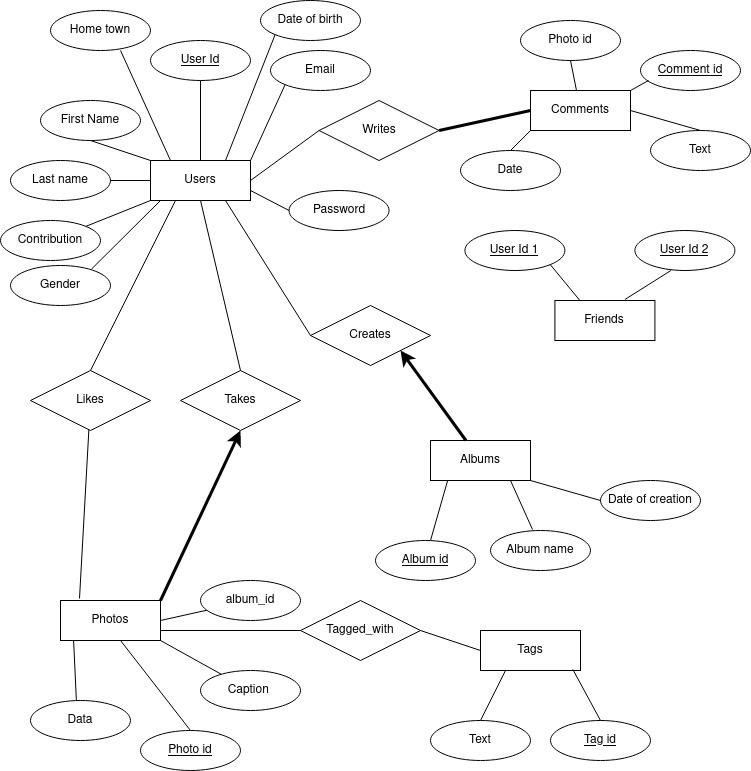
\includegraphics[width=6.5in, height=9in]{ER_diagram}

  \section{Assumptions}
  In the Users table, we store a password hash to avoid storing cleartext
  passwords.  In testing with SHA-256 encryption, as suggested on Piazza, this
  hash appears to be just short of 80 characters.  It would be bad to
  accidentally mutilate the hash, however, so this field has some extra space,
  just in case.

  In the final section of the schema, we have several triggers to easily update
  a user's contribution score.  The removal triggers, in particular, are hooked
  up to the appropriate relationship tables, because it would be unfair for a
  user to maintain their high contribution score if they were to delete a great
  number of their photos, or if others delete photos on which they have
  commented, because there would then no longer be proof of their contributions.

  Using only SQL, it is difficult to prevent a user from commenting on their own
  photo.  As such, this logic will have to be implemented in Flask instead.
  This does incur some lag for the end-user, but that's preferable to writing
  convoluted SQL in an attempt to make the language perform a task for which it
  was never designed.

  Using only SQL, it is also difficult to make sure that a user cannot become
  friends with themselves somehow.  Obviously, no one should be able to befriend
  themselves, because that makes no sense.  However, SQL treats a set of columns
  (1, 2) as identical to the set (2, 1), which goes against the application's
  semantics.  So this, too, will have to be done in Python.

  In addition to the entity and relationship tables, we have created a view to
  calculate the users with the highest contribution scores.  We could have
  stored this as a true table, but contribution scores are likely to change
  quickly.  As such, it makes more sense to just recalculate the top-10 list on
  the fly, saving us the effort of constantly keeping another table up-to-date.
\end{document}
